\begin{frame}{detectMultiScale in Viola-Jones (or \texttt{CascadeClassifier})}
  \footnotesize
  \centering
  \vspace{1em}

  \begin{columns}
    \column{0.4\textwidth}

    The Viola-Jones \cite{viola2001rapid} object detection framework is a
    generic framework for object detection, which is particularly successful for
    face detection.

    \begin{itemize}
      \visible<2->{
      \item \texttt{scale}: how much the image size is reduced at each image
        scale.
      \item \texttt{min\_size}: minimum detect-able object size.
      }
      \visible<3>{
      \item \texttt{min\_neighbors}: how many neighbors each candidate rectangle
        should have to retain it.
      }
    \end{itemize}

    \column{0.6\textwidth}

    \only<2>{
      \begin{figure}
        \centering
        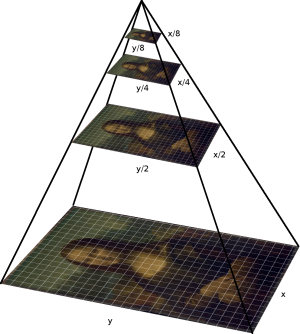
\includegraphics[width=0.95\linewidth]{figures/vj-scale.png}
        \caption{Image Source: pyimagesearch.}
      \end{figure}
    }

    \only<3->{
      \begin{figure}
        \centering
        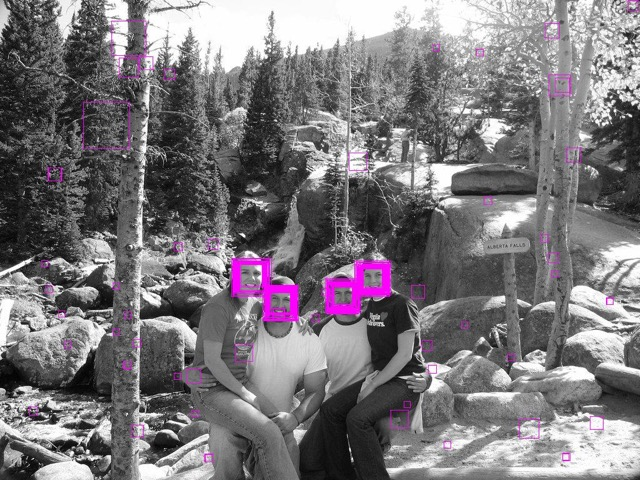
\includegraphics[width=0.7\linewidth]{figures/min_neighbors-1.jpg} \\
        \vspace{0.5em}
        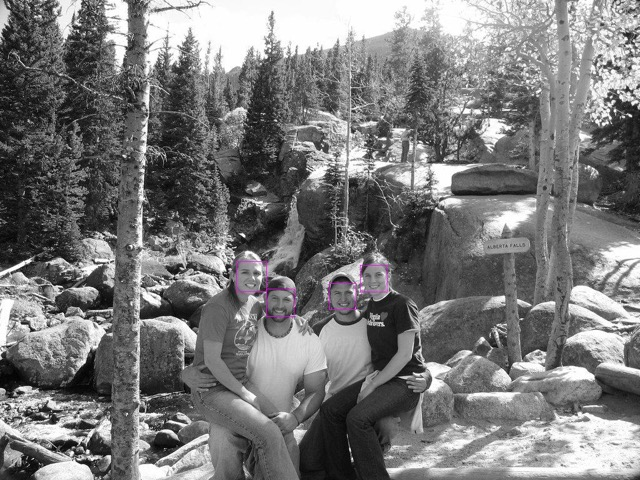
\includegraphics[width=0.7\linewidth]{figures/min_neighbors-3.jpg}
        \caption{Image Source: Stack Overflow.}
      \end{figure}
    }
  \end{columns}
\end{frame}

\begin{frame}[fragile]{detectMultiScale in Histogram of Oriented Gradients (HOG)}
  \vspace{1em}
  \centering
\begin{Verbatim}[fontsize=\scriptsize]
pub struct HogParams {
    pub win_size: Size2i,
    pub block_size: Size2i,
    pub block_stride: Size2i,
    pub cell_size: Size2i,
    pub nbins: c_int,
    pub win_sigma: f64,
    pub l2hys_threshold: f64,
    pub gamma_correction: bool,
    pub nlevels: usize,
    pub hit_threshold: f64,
    pub win_stride: Size2i,
    pub padding: Size2i,
    pub scale: f64,
    pub group_threshold: c_int,
    pub use_meanshift_grouping: bool,
    pub final_threshold: f64,
}
\end{Verbatim}
\end{frame}

\begin{frame}{Exhaustive Search is Too Expensive}
  \vspace{1em}
  \begin{figure}
    \centering
    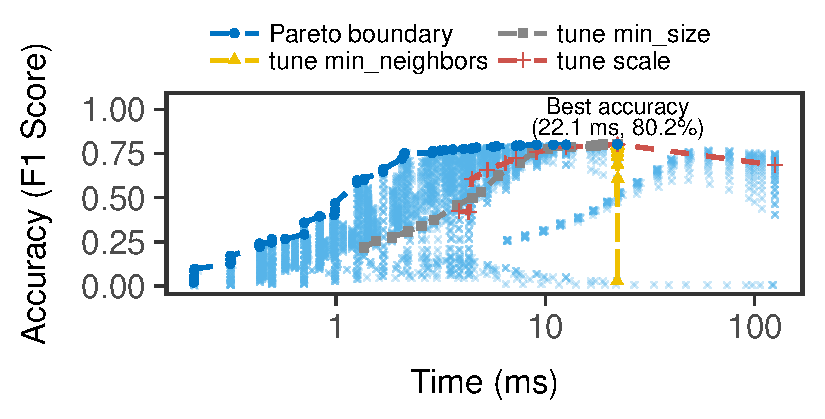
\includegraphics[width=0.8\linewidth]{figures/serving-eval-exhaustive.pdf}
  \end{figure}

  \begin{itemize}
    \item \texttt{scale}: how much the image size is reduced at each image
      scale.
    \item \texttt{min\_size}: minimum detect-able object size.
    \item \texttt{min\_neighbors}: how many neighbors each candidate rectangle
      should have to retain it.
  \end{itemize}
\end{frame}

%%% Local Variables:
%%% mode: latex
%%% TeX-master: "../talk"
%%% TeX-engine: xetex
%%% End:
